% TrustRAG defense as applied in the poisonedrag-modern PoisonedRAG pipeline (NQ, Step 5).
% TikZ port of trustrag_architecture.svg: same coordinates (x = 1pt, y = -1pt, so SVG px map 1:1 and y points down),
% same text sizes, same palette. The picture is 1200pt wide; scale it in a paper with
%   \includegraphics[width=\textwidth]{trustrag_architecture.pdf}        (after compiling this file), or
%   \resizebox{\textwidth}{!}{<the tikzpicture below>}                   (copy the preamble macros too).
% \figcaptionfalse drops the built-in caption and footnotes (use \caption{...} in the paper instead).
% Build: pdflatex trustrag_architecture.tex   (TeX Live 2022: tikz arrows.meta + patterns.meta, helvet)
% Numbers: experiments/RESULTS.md Step 5 (D1-D3, Limitations); experiments/defenses/trustrag_filter_simcse_*.json.
\documentclass[tikz,border=2pt]{standalone}
\usepackage{fix-cm}           % scalable Computer Modern for the math arrows at any size
\usepackage[T1]{fontenc}
\usepackage{helvet}
\usepackage{courier}          % Type 1 typewriter (avoids bitmap EC fonts)
\renewcommand{\familydefault}{\sfdefault}
\usepackage{textcomp}
\usetikzlibrary{arrows.meta,patterns.meta}

\newif\iffigcaption \figcaptiontrue

% ---- palette (matches the SVG and app/pages/1_Architecture.py) ----
\definecolor{ink}{HTML}{1F1E1C}       \definecolor{ink2}{HTML}{55534E}     \definecolor{ink3}{HTML}{7A7873}
\definecolor{poison}{HTML}{E34948}    \definecolor{poisondark}{HTML}{A8302F} \definecolor{poisonchip}{HTML}{8F2423}
\definecolor{poisontint}{HTML}{FDE8E8} \definecolor{poisonsoft}{HTML}{FDEEEE} \definecolor{hatchsoft}{HTML}{F0A09F}
\definecolor{clean}{HTML}{1BAF7A}     \definecolor{cleandark}{HTML}{127552} \definecolor{cleanchip}{HTML}{D3EFE2}
\definecolor{cleantint}{HTML}{E3F6EE}
\definecolor{model}{HTML}{2A78D6}     \definecolor{modeltint}{HTML}{E1ECFA} \definecolor{modelbg}{HTML}{F4F8FD}
\definecolor{neutral}{HTML}{8A8984}   \definecolor{neutraltint}{HTML}{F0EFEC}
\definecolor{flowc}{HTML}{4A4842}     \definecolor{badge}{HTML}{3D3C39}     \definecolor{defense}{HTML}{F6F3EA}
\definecolor{kbfill}{HTML}{FBFAF7}    \definecolor{outcome}{HTML}{FBF7F6}   \definecolor{legendline}{HTML}{D6D4CF}
\definecolor{caveatfill}{HTML}{FFF8E6} \definecolor{caveatline}{HTML}{B7791F}
\definecolor{amber}{HTML}{F2B632}     \definecolor{amberdark}{HTML}{8A5A0B} \definecolor{warnink}{HTML}{3D2A05}

\newcommand{\fs}[1]{\fontsize{#1}{#1}\selectfont}
\newcommand{\arr}{\ensuremath{\rightarrow}}
\newcommand{\mdot}{\textperiodcentered}

\tikzset{
  t/.style={anchor=base west, inner sep=0pt, outer sep=0pt, text=ink},
  tc/.style={anchor=base, inner sep=0pt, outer sep=0pt, text=ink},
  te/.style={anchor=base east, inner sep=0pt, outer sep=0pt, text=ink},
  s/.style={font=\fs{12}}, b/.style={font=\fs{12.5}},
  h3/.style={font=\fs{13}\bfseries}, h2/.style={font=\fs{15}\bfseries}, h1/.style={font=\fs{17}\bfseries},
  tip/.tip={Triangle[length=8pt,width=7.2pt]},
  flow/.style={draw=flowc, line width=1.4pt, -tip},
  byp/.style={draw=flowc, line width=1.3pt, dash pattern=on 4pt off 3pt},
  call/.style={draw=model, line width=1.3pt, dash pattern=on 5pt off 3pt, {Triangle[length=7pt,width=6.3pt]}-{Triangle[length=7pt,width=6.3pt]}},
  box/.style={line width=1.1pt, rounded corners=6pt},
  hatch/.style={preaction={fill=poisontint}, pattern={Lines[angle=45,distance=5pt,line width=2pt]}, pattern color=poison,
                draw=poison, line width=1.1pt},
  hatchsoft/.style={preaction={fill=poisonsoft}, pattern={Lines[angle=45,distance=6pt,line width=1.6pt]}, pattern color=hatchsoft},
}
\newcommand{\badge}[3]{\fill[badge] (#1,#2) circle[radius=10];
  \node[tc, text=white, font=\fs{12.5}\bfseries] at (#1,#2+4.5) {#3};}
\newcommand{\lbadge}[3]{\draw[fill=white, draw=badge, line width=1.2pt] (#1,#2) circle[radius=8];
  \node[tc, font=\fs{11}\bfseries] at (#1,#2+4) {#3};}
\newcommand{\tri}[2]{\filldraw[fill=poison, draw=poisondark, line width=0.8pt, line join=round, shift={(#1,#2)}]
  (5,0.5) -- (9.5,8.5) -- (0.5,8.5) -- cycle;}
\newcommand{\warn}[3]{\begin{scope}[shift={(#1,#2)}, scale=#3]
  \filldraw[fill=amber, draw=amberdark, line width=1pt, line join=round] (8,0.8) -- (15.3,13.3) -- (0.7,13.3) -- cycle;
  \fill[warnink] (7.2,4.4) rectangle ++(1.6,5); \fill[warnink] (7.2,10.4) rectangle ++(1.6,1.6);
  \end{scope}}
\newcommand{\checkmk}[2]{\draw[cleandark, line width=1.4pt, line cap=round, line join=round] (#1,#2) -- ++(2.5,2.5) -- ++(5,-5);}

\begin{document}
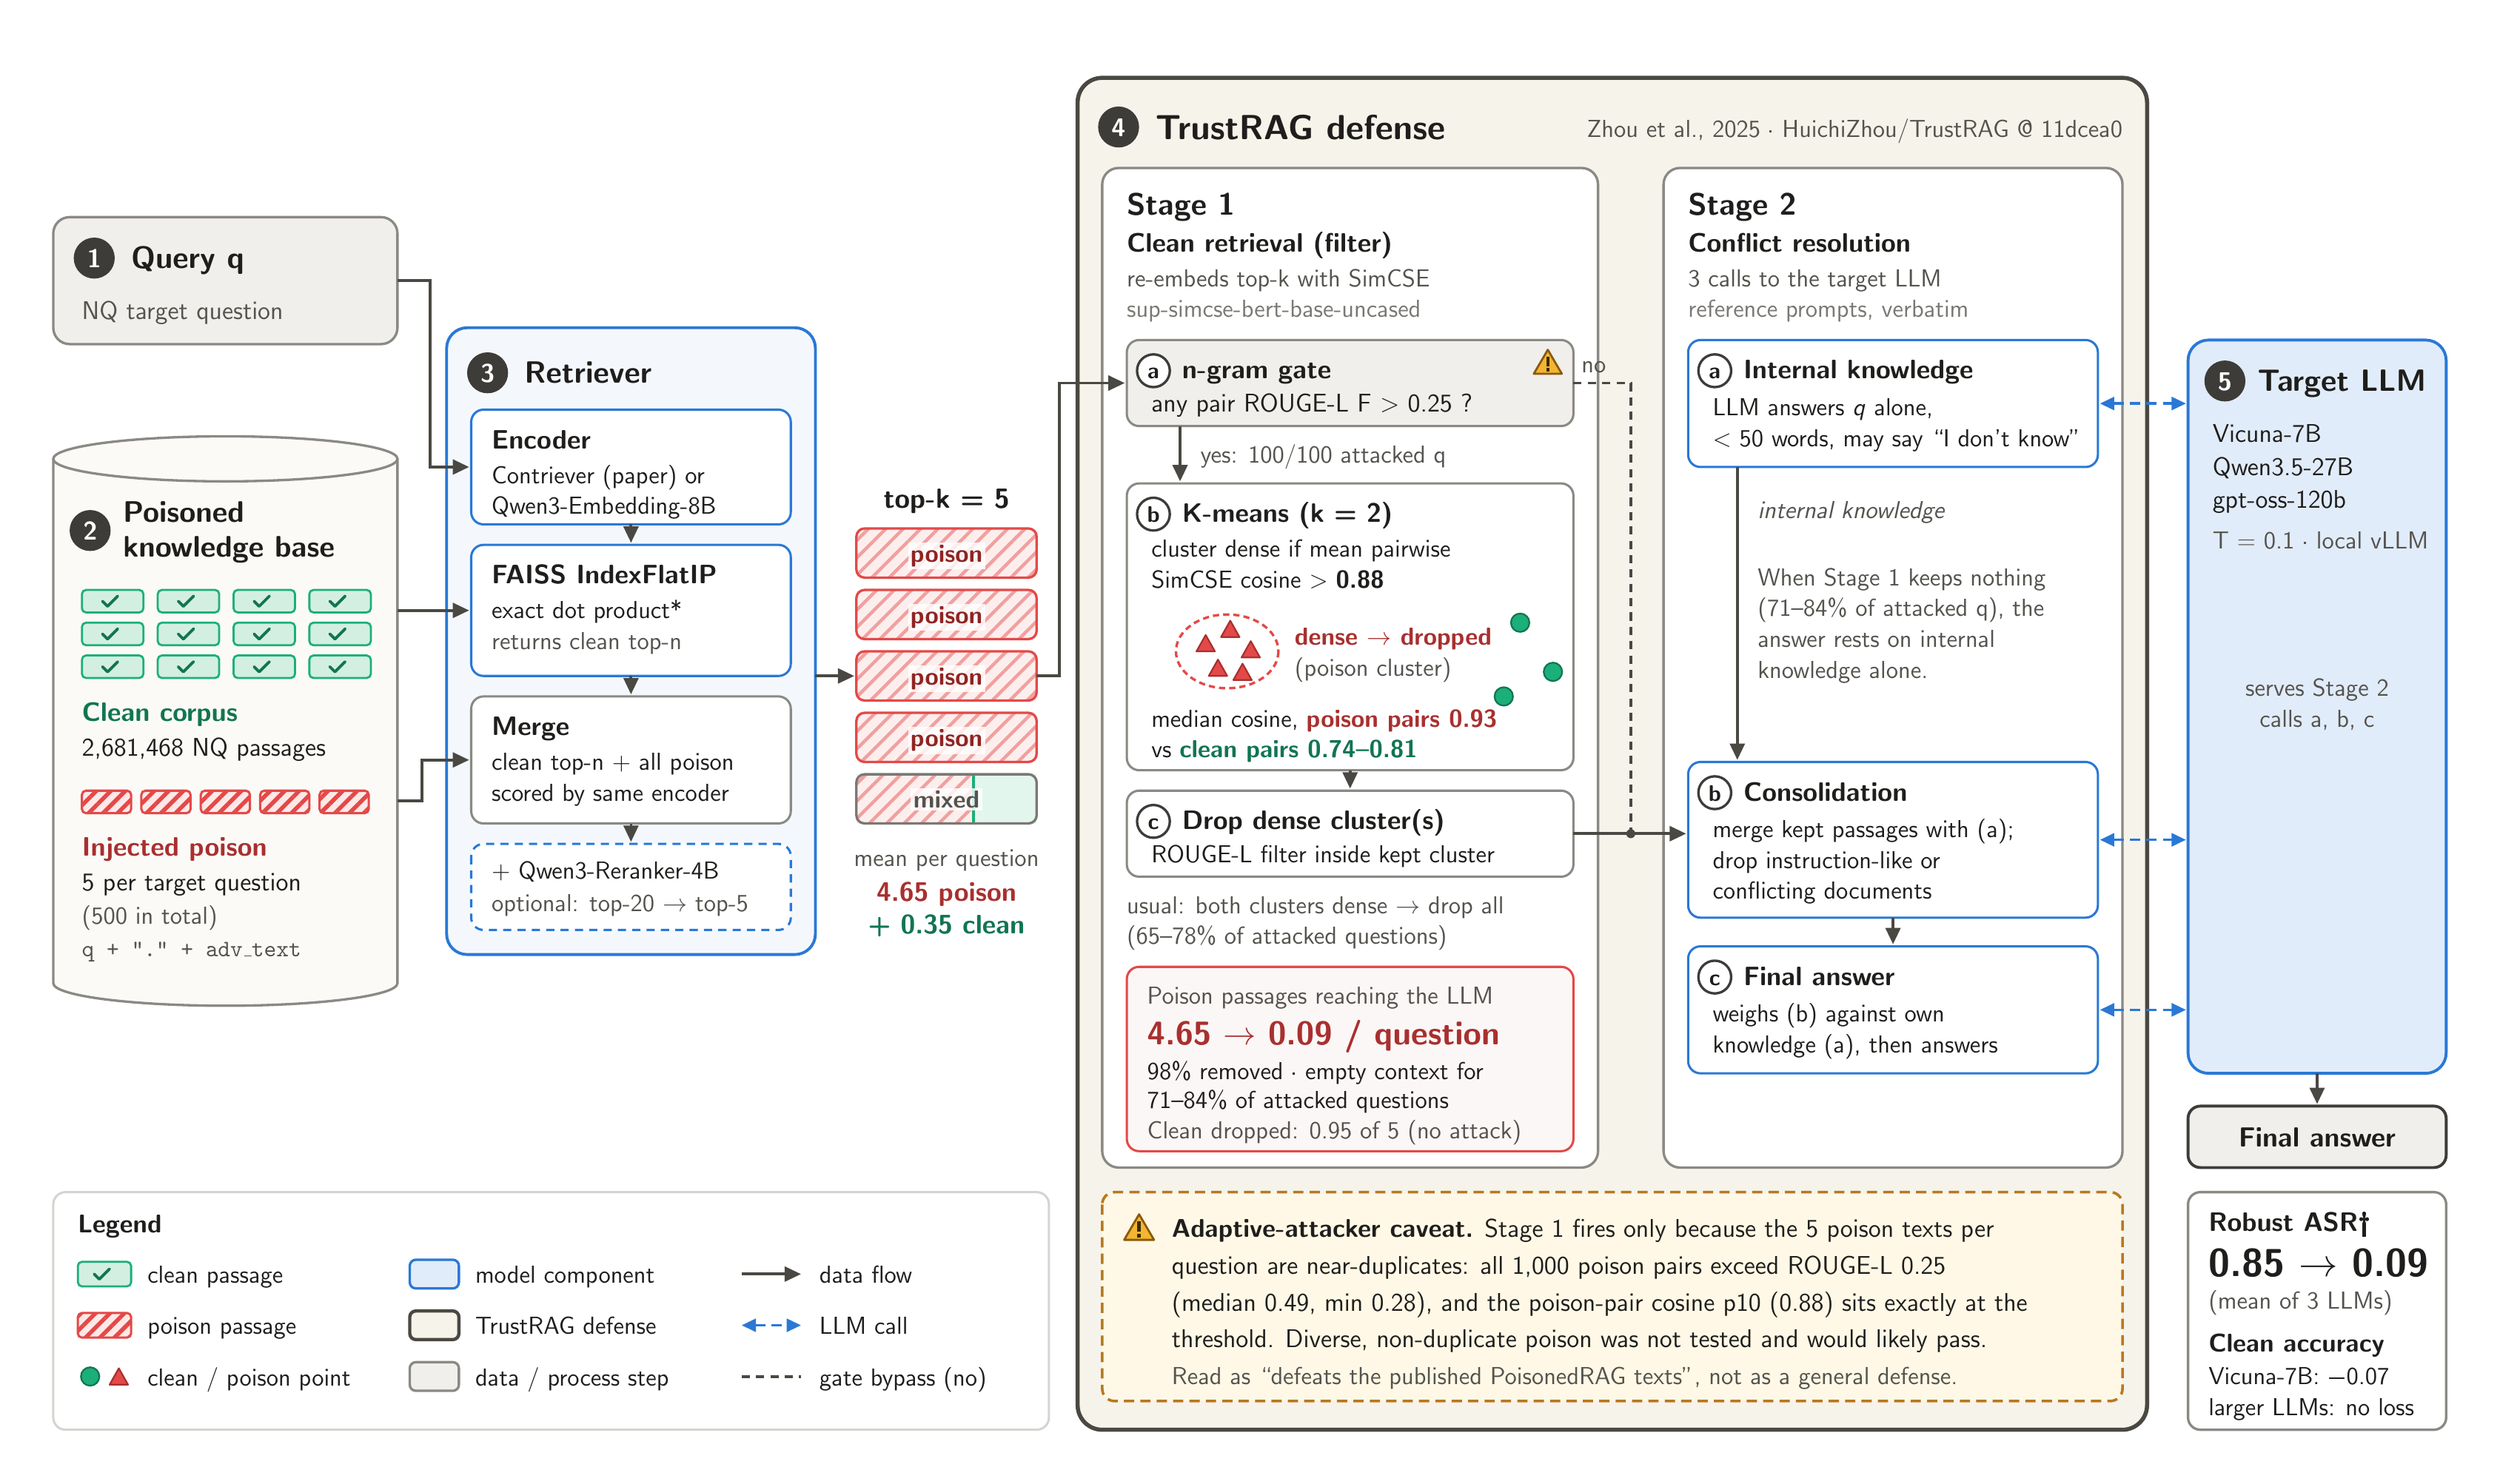
\begin{tikzpicture}[x=1pt, y=-1pt]
  % canvas (keeps the bounding box identical to the SVG)
  \iffigcaption \fill[white] (0,0) rectangle (1200,796); \else \fill[white] (0,0) rectangle (1200,696); \fi

  % ===== 1 · Query =====
  \draw[neutral, fill=neutraltint, line width=1.2pt, rounded corners=8pt] (16,96) rectangle (184,158);
  \badge{36}{116}{1}
  \node[t, h2] at (54,121) {Query \textit{q}};
  \node[t, b, text=ink2] at (30,146) {NQ target question};

  % ===== 2 · Poisoned knowledge base =====
  \filldraw[fill=kbfill, draw=neutral, line width=1.2pt]
    (16,214) -- (16,470) arc[start angle=180, end angle=0, x radius=84, y radius=11]
    -- (184,214) arc[start angle=0, end angle=-180, x radius=84, y radius=11] -- cycle;
  \draw[neutral, line width=1.2pt] (16,214) arc[start angle=180, end angle=0, x radius=84, y radius=11];
  \badge{34}{249}{2}
  \node[t, font=\fs{14.5}\bfseries] at (50,245) {Poisoned};
  \node[t, font=\fs{14.5}\bfseries] at (50,262) {knowledge base};
  \foreach \x in {30,67,104,141} \foreach \y in {278,294,310} {
    \draw[clean, fill=cleanchip, line width=1pt, rounded corners=2pt] (\x,\y) rectangle ++(30,11);
    \checkmk{\x+10}{\y+5.5}}
  \node[t, h3, text=cleandark] at (30,342) {Clean corpus};
  \node[t, b] at (30,359) {2,681,468 NQ passages};
  \foreach \x in {30,59,88,117,146} \path[hatch, rounded corners=2pt] (\x,376) rectangle ++(24,11);
  \node[t, h3, text=poisondark] at (30,408) {Injected poison};
  \node[t, b] at (30,425) {5 per target question};
  \node[t, s, text=ink2] at (30,441) {(500 in total)};
  \node[t, font=\fs{11.5}\ttfamily, text=ink2] at (30,457) {q + "." + adv\_text};

  % ===== 3 · Retriever =====
  \draw[model, fill=modelbg, line width=1.4pt, rounded corners=10pt] (208,150) rectangle (388,456);
  \badge{228}{172}{3}
  \node[t, h2] at (246,177) {Retriever};
  \draw[box, model, fill=white] (220,190) rectangle (376,246);
  \node[t, h3] at (230,209) {Encoder};
  \node[t, s] at (230,226) {Contriever (paper) or};
  \node[t, s] at (230,241) {Qwen3-Embedding-8B};
  \draw[box, model, fill=white] (220,256) rectangle (376,320);
  \node[t, h3] at (230,275) {FAISS IndexFlatIP};
  \node[t, s] at (230,292) {exact dot product*};
  \node[t, s, text=ink2] at (230,307) {returns clean top-n};
  \draw[box, neutral, fill=white] (220,330) rectangle (376,392);
  \node[t, h3] at (230,349) {Merge};
  \node[t, s] at (230,366) {clean top-n + all poison};
  \node[t, s] at (230,381) {scored by same encoder};
  \draw[box, model, fill=white, dash pattern=on 4pt off 3pt] (220,402) rectangle (376,444);
  \node[t, s] at (230,419) {+ Qwen3-Reranker-4B};
  \node[t, s, text=ink2] at (230,435) {optional: top-20 \arr{} top-5};
  \draw[flow] (298,246) -- (298,255);
  \draw[flow] (298,320) -- (298,329);
  \draw[byp, -tip] (298,392) -- (298,401);
  % inputs
  \draw[flow] (184,127) -- (200,127) -- (200,218) -- (219,218);
  \draw[flow] (184,288) -- (219,288);
  \draw[flow] (184,381) -- (196,381) -- (196,361) -- (219,361);

  % ===== retrieved top-k =====
  \draw[flow] (388,320) -- (407,320);
  \node[tc, font=\fs{13.5}\bfseries] at (452,238) {top-k = 5};
  \foreach \y in {248,278,308,338} {
    \path[hatchsoft, rounded corners=4pt] (408,\y) rectangle ++(88,24);
    \draw[poison, line width=1.2pt, rounded corners=4pt] (408,\y) rectangle ++(88,24);
    \node[tc, font=\fs{12}\bfseries, text=poisonchip, fill=white, fill opacity=0.8, text opacity=1, inner sep=1.2pt]
      at (452,\y+16.5) {poison};}
  \path[hatchsoft] (408,368) rectangle (465.2,392);
  \fill[cleantint] (465.2,368) rectangle (496,392);
  \draw[clean, line width=1.2pt] (465.2,368) -- (465.2,392);
  \draw[ink3, line width=1.2pt, rounded corners=4pt] (408,368) rectangle (496,392);
  \node[tc, font=\fs{12}\bfseries, text=ink2, fill=white, fill opacity=0.8, text opacity=1, inner sep=1.2pt] at (452,384.5) {mixed};
  \node[tc, s, text=ink2] at (452,413) {mean per question};
  \node[tc, h3, text=poisondark] at (452,430) {4.65 poison};
  \node[tc, h3, text=cleandark] at (452,446) {+ 0.35 clean};

  % ===== 4 · TrustRAG defense =====
  \draw[flowc, fill=defense, line width=2pt, rounded corners=12pt] (516,28) rectangle (1038,688);
  \badge{536}{52}{4}
  \node[t, h1] at (554,58) {TrustRAG defense};
  \node[te, s, text=ink2] at (1026,57) {Zhou et al., 2025 \mdot{} HuichiZhou/TrustRAG @ 11dcea0};

  % --- Stage 1 ---
  \draw[neutral, fill=white, line width=1.2pt, rounded corners=8pt] (528,72) rectangle (770,560);
  \node[t, h2] at (540,95) {Stage 1};
  \node[t, h3] at (540,113) {Clean retrieval (filter)};
  \node[t, s, text=ink2] at (540,130) {re-embeds top-k with SimCSE};
  \node[t, s, text=ink3] at (540,145) {sup-simcse-bert-base-uncased};
  % a · gate
  \draw[box, neutral, fill=neutraltint] (540,156) rectangle (758,198);
  \lbadge{553}{171}{a}
  \node[t, h3] at (567,175) {n-gram gate};
  \node[t, b] at (552,191) {any pair ROUGE-L F \textgreater{} 0.25 ?};
  \warn{738}{160}{0.9375}
  \draw[flow] (566,198) -- (566,225);
  \node[t, s, text=ink2] at (576,216) {yes: 100/100 attacked q};
  \draw[byp] (758,177) -- (786,177) -- (786,397);
  \node[t, s, text=ink2] at (762,172) {no};
  % b · K-means
  \draw[box, neutral, fill=white] (540,226) rectangle (758,366);
  \lbadge{553}{241}{b}
  \node[t, h3] at (567,245) {K-means (k = 2)};
  \node[t, s] at (552,262) {cluster dense if mean pairwise};
  \node[t, s] at (552,277) {SimCSE cosine \textgreater{} \textbf{0.88}};
  \draw[poison, line width=1.2pt, dash pattern=on 3pt off 2pt] (589,308) ellipse[x radius=25, y radius=18];
  \tri{573.5}{299.5} \tri{585.5}{292.5} \tri{595.5}{302.5} \tri{579.5}{311.5} \tri{591.5}{313.5}
  \node[t, font=\fs{12}\bfseries, text=poisondark] at (622,305) {dense \arr{} dropped};
  \node[t, s, text=ink2] at (622,320) {(poison cluster)};
  \foreach \p in {(732,294),(748,318),(724,330)} \filldraw[fill=clean, draw=cleandark, line width=0.8pt] \p circle[radius=4.5];
  \node[t, s] at (552,345) {median cosine, \textcolor{poisondark}{\bfseries poison pairs 0.93}};
  \node[t, s] at (552,360) {vs \textcolor{cleandark}{\bfseries clean pairs 0.74--0.81}};
  \draw[flow] (649,366) -- (649,375);
  % c · drop
  \draw[box, neutral, fill=white] (540,376) rectangle (758,418);
  \lbadge{553}{391}{c}
  \node[t, h3] at (567,395) {Drop dense cluster(s)};
  \node[t, s] at (552,411) {ROUGE-L filter inside kept cluster};
  \node[t, s, text=ink2] at (540,436) {usual: both clusters dense \arr{} drop all};
  \node[t, s, text=ink2] at (540,451) {(65--78\% of attacked questions)};
  % outcome
  \draw[box, poison, fill=outcome] (540,462) rectangle (758,552);
  \node[t, s, text=ink2] at (550,480) {Poison passages reaching the LLM};
  \node[t, font=\fs{16}\bfseries, text=poisondark] at (550,500) {4.65 \arr{} 0.09 / question};
  \node[t, s] at (550,517) {98\% removed \mdot{} empty context for};
  \node[t, s] at (550,531) {71--84\% of attacked questions};
  \node[t, s, text=ink2] at (550,546) {Clean dropped: 0.95 of 5 (no attack)};

  % --- Stage 2 ---
  \draw[neutral, fill=white, line width=1.2pt, rounded corners=8pt] (802,72) rectangle (1026,560);
  \node[t, h2] at (814,95) {Stage 2};
  \node[t, h3] at (814,113) {Conflict resolution};
  \node[t, s, text=ink2] at (814,130) {3 calls to the target LLM};
  \node[t, s, text=ink3] at (814,145) {reference prompts, verbatim};
  % a · internal knowledge
  \draw[box, model, fill=white] (814,156) rectangle (1014,218);
  \lbadge{827}{171}{a}
  \node[t, h3] at (841,175) {Internal knowledge};
  \node[t, s] at (826,193) {LLM answers \textit{q} alone,};
  \node[t, s] at (826,208) {\textless{} 50 words, may say \textquotedblleft I don't know\textquotedblright};
  \draw[flow] (838,218) -- (838,361);
  \node[t, s, text=ink2, font=\fs{12}\itshape] at (848,243) {internal knowledge};
  \node[t, s, text=ink2] at (848,276) {When Stage 1 keeps nothing};
  \node[t, s, text=ink2] at (848,291) {(71--84\% of attacked q), the};
  \node[t, s, text=ink2] at (848,306) {answer rests on internal};
  \node[t, s, text=ink2] at (848,321) {knowledge alone.};
  % b · consolidation
  \draw[box, model, fill=white] (814,362) rectangle (1014,438);
  \lbadge{827}{377}{b}
  \node[t, h3] at (841,381) {Consolidation};
  \node[t, s] at (826,399) {merge kept passages with (a);};
  \node[t, s] at (826,414) {drop instruction-like or};
  \node[t, s] at (826,429) {conflicting documents};
  \draw[flow] (914,438) -- (914,451);
  % c · final answer
  \draw[box, model, fill=white] (814,452) rectangle (1014,514);
  \lbadge{827}{467}{c}
  \node[t, h3] at (841,471) {Final answer};
  \node[t, s] at (826,489) {weighs (b) against own};
  \node[t, s] at (826,504) {knowledge (a), then answers};

  % caveat
  \draw[caveatline, fill=caveatfill, line width=1.3pt, dash pattern=on 5pt off 3pt, rounded corners=6pt] (528,572) rectangle (1026,674);
  \warn{538}{582}{1}
  \node[t, b] at (562,594) {\textbf{Adaptive-attacker caveat.} Stage 1 fires only because the 5 poison texts per};
  \node[t, b] at (562,612) {question are near-duplicates: all 1,000 poison pairs exceed ROUGE-L 0.25};
  \node[t, b] at (562,630) {(median 0.49, min 0.28), and the poison-pair cosine p10 (0.88) sits exactly at the};
  \node[t, b] at (562,648) {threshold. Diverse, non-duplicate poison was not tested and would likely pass.};
  \node[t, s, text=ink2] at (562,666) {Read as \textquotedblleft defeats the published PoisonedRAG texts\textquotedblright, not as a general defense.};

  % ===== 5 · Target LLM -> final answer =====
  \draw[model, fill=modeltint, line width=1.4pt, rounded corners=10pt] (1058,156) rectangle (1184,514);
  \badge{1076}{176}{5}
  \node[t, h2] at (1092,181) {Target LLM};
  \node[t, b] at (1070,206) {Vicuna-7B};
  \node[t, b] at (1070,222) {Qwen3.5-27B};
  \node[t, b] at (1070,238) {gpt-oss-120b};
  \node[t, s, text=ink2] at (1070,258) {T = 0.1 \mdot{} local vLLM};
  \node[tc, s, text=ink2] at (1121,330) {serves Stage 2};
  \node[tc, s, text=ink2] at (1121,345) {calls a, b, c};
  \draw[call] (1015,187) -- (1057,187);
  \draw[call] (1015,400) -- (1057,400);
  \draw[call] (1015,483) -- (1057,483);
  \draw[flow] (1121,514) -- (1121,529);
  \draw[badge, fill=neutraltint, line width=1.4pt, rounded corners=6pt] (1058,530) rectangle (1184,560);
  \node[tc, font=\fs{13.5}\bfseries] at (1121,550) {Final answer};
  \draw[neutral, fill=white, line width=1.2pt, rounded corners=6pt] (1058,572) rectangle (1184,688);
  \node[t, h3] at (1068,591) {Robust ASR\textdagger};
  \node[t, font=\fs{19}\bfseries] at (1068,613) {0.85 \arr{} 0.09};
  \node[t, s, text=ink2] at (1068,629) {(mean of 3 LLMs)};
  \node[t, font=\fs{12.5}\bfseries] at (1068,650) {Clean accuracy};
  \node[t, s] at (1068,666) {Vicuna-7B: \textminus 0.07};
  \node[t, s] at (1068,681) {larger LLMs: no loss};

  % ===== legend =====
  \draw[legendline, fill=white, line width=1.1pt, rounded corners=6pt] (16,572) rectangle (502,688);
  \node[t, font=\fs{12.5}\bfseries] at (28,592) {Legend};
  \draw[clean, fill=cleanchip, line width=1pt, rounded corners=2pt] (28,606) rectangle ++(26,12);
  \checkmk{36}{612}
  \node[t, s] at (62,616.5) {clean passage};
  \path[hatch, rounded corners=2pt] (28,631) rectangle ++(26,12);
  \node[t, s] at (62,641.5) {poison passage};
  \filldraw[fill=clean, draw=cleandark, line width=0.8pt] (34,662) circle[radius=4.5];
  \tri{43}{657.5}
  \node[t, s] at (62,666.5) {clean / poison point};
  \draw[model, fill=modeltint, line width=1.2pt, rounded corners=3pt] (190,605) rectangle ++(24,14);
  \node[t, s] at (222,616.5) {model component};
  \draw[flowc, fill=defense, line width=1.6pt, rounded corners=3pt] (190,630) rectangle ++(24,14);
  \node[t, s] at (222,641.5) {TrustRAG defense};
  \draw[neutral, fill=neutraltint, line width=1.2pt, rounded corners=3pt] (190,655) rectangle ++(24,14);
  \node[t, s] at (222,666.5) {data / process step};
  \draw[flow] (352,612) -- (381,612);
  \node[t, s] at (390,616.5) {data flow};
  \draw[call] (352,637) -- (381,637);
  \node[t, s] at (390,641.5) {LLM call};
  \draw[byp] (352,662) -- (381,662);
  \node[t, s] at (390,666.5) {gate bypass (no)};

  % ===== connectors drawn last =====
  \draw[flow] (496,320) -- (507,320) -- (507,177) -- (539,177);
  \draw[flow] (758,397) -- (813,397);
  \fill[flowc] (786,397) circle[radius=2.2];

  % ===== caption =====
  \iffigcaption
  \node[t, font=\fs{13}] at (16,716) {\textbf{Figure 1.} TrustRAG as deployed in our PoisonedRAG pipeline (BEIR NQ, full 100-question protocol, top-k = 5, N = 5 poison texts per question; means over 3 retrieval setups \texttimes{} 3 LLMs): Stage 1 removes};
  \node[t, font=\fs{13}] at (16,733) {the near-duplicate poison cluster (4.65 \arr{} 0.09 poison passages per question) and Stage 2 reconciles what remains with the LLM's own knowledge, cutting robust ASR from 0.85 to 0.09; only Vicuna-7B};
  \node[t, font=\fs{13}] at (16,750) {loses clean accuracy (\textminus 0.07).};
  \node[t, font=\fs{11.5}, text=ink2] at (16,771) {\textdagger{} Robust ASR = exact match for Vicuna-7B, answered-only for Qwen3.5-27B, typography-normalized for gpt-oss-120b (per LLM 0.85 \arr{} 0.09, 0.90 \arr{} 0.08, 0.79 \arr{} 0.09). * Contriever cells use upstream's precomputed BEIR};
  \node[t, font=\fs{11.5}, text=ink2] at (16,786) {top-100 instead of FAISS (same top-k on 100/100 questions). Sources: experiments/RESULTS.md Step 5 (Tables D1--D3) and experiments/defenses/trustrag\_filter\_simcse\_*.json.};
  \fi
\end{tikzpicture}
\end{document}
